% ---------------------
% EXPERIMENTATION ET RESULTATS
% ---------------------
\chapter{Expérimentations et résultats} \label{ch_five}

\section{Protocole expérimental et métriques}

\subsection{Configuration matérielle et logicielle}

L'ensemble des expérimentations rapportées dans ce chapitre ont été réalisées sur une station de travail équipée de 2 GPU NVIDIA RTX A5000 (24 Go GDDR6 ECC, architecture Ampere), d'un CPU AMD Ryzen Threadripper PRO 5965WX 24-Cores et de 128 Go de mémoire RAM. L'environnement logiciel repose sur Ubuntu 22.04.3 LTS (Jammy Jellyfish), CUDA 12.2 (Driver Version: 535.154.05). Les différentes bibliothèques utilisées sont toutes présentes dans le fichier \emph{pixi.toml} présent à la racine du projet. Elles ne sont pas citées ici car elle dépendent de l'environement choisit lors des exécutions des différents modules.

L'ensemble de la chaîne expérimentale est versionnée sous Git (voir annexe~\ref{ann:reproducibility}) les checkpoints sont à téléchargés via des liens présents dans le fichier \emph{README.md} à la racine du projet, garantissant la reproductibilité de chaque exécution. Des graines aléatoires (\emph{seeds}) ont été utilisées pour l'initialisation LoRA mais aussi pour la partition du dataset de fine-tuning, assurant la reproductibilité des résultats.

Le suivi des expérimentations est assuré via Weights \& Biases (wandb)~\cite{wandb}, qui enregistre les métriques de validation (SSIM, LPIPS) et la fonction de perte (loss) à chaque checkpoint.

\subsection*{Remarque sur le protocole de test}

Les trois séquences du jeu de données de test sont issues d'un sujet dont les vidéos ont été reçues après la constitution du dataset et la réalisation du fine-tuning. Ce sujet est donc absent de l'ensemble des données d'entraînement et de validation, garantissant une évaluation de la capacité de généralisation du modèle à des morphologies et des conditions de capture non vues. Les occlusions synthétiques ont été générées via le même pipeline que celui utilisé pour le dataset d'entraînement, assurant la cohérence du protocole d'évaluation.

\subsection{Métriques d'évaluation}

Les deux métriques introduites au chapitre~\ref{ch_four} (SSIM, LPIPS) sont utilisées pour l'évaluation quantitative. Pour chaque clip du jeu de données de test, chaque métrique est calculée comme suit :

\begin{itemize}
  \item Calcul trame-par-trame entre la sortie reconstruite et la référence, restreint aux régions occluses.
  \item Moyennage temporel sur l'ensemble des trames du clip.
  \item Moyennage final sur l'ensemble des clips du jeu de données de test, accompagné de l'écart-type pour caractériser la dispersion.
\end{itemize}

Les implémentations utilisées sont les implémentations de référence de \texttt{torchmetrics}~\cite{Torchmetrics-2022} pour SSIM, et l'implémentation officielle de \texttt{lpips}~\cite{LPIPS-2018} avec backbone AlexNet pour LPIPS.

\subsection{Modèles comparés}

Deux configurations sont systématiquement comparées :

\begin{enumerate}
  \item \textbf{TACO-baseline.} Le modèle TACO pré-entraîné par les auteurs, utilisé tel quel sans adaptation.
  \item \textbf{TACO-LoRA.} Le modèle obtenu par fine-tuning LoRA sur le dataset spécialisé décrit au chapitre~\ref{ch_four}.
\end{enumerate}

\section{Courbes d'entraînement}

L'évolution de la fonction de perte (\textit{loss}), présente des oscillations autour de la médiane qui est de $0{,}013$ avec des pics ponctuels (figure~\ref{fig:courbe-loss-lpips-ssim}) : atteignant $0{,}058$ à l'étape 949, $0{,}077$ à l'étape 2\,149 et $0{,}097$ à l'étape 2\,899, sans pour autant diverger. Ce comportement est caractéristique d'un fine-tuning sur un dataset de petite taille et peut indiquer un taux d'apprentissage légèrement supra-optimal pour certains mini-batchs~\cite{LoRA-2021}.

L'évolution de la LPIPS de validation constitue le signal le plus informatif (figure~\ref{fig:courbe-loss-lpips-ssim}). Il débute à $0{,}0205$ à l'étape 34, atteint un pic transitoire de $0{,}0269$ à l'étape 170 (correspondant à la phase d'adaptation initiale des adaptateurs LoRA), puis décroît régulièrement pour se stabiliser autour de $0{,}0181$ sur la phase stable (étapes 1\,500 à 3\,400). Le minimum absolu de $0{,}0168$ est atteint à l'étape 2\,754. La réduction totale de 12,3\,\% par rapport à la valeur initiale confirme l'adaptation effective du modèle au domaine de la force athlétique.

L'évolution de la SSIM de validation progresse de $0{,}982$ au premier checkpoint à $0{,}985$ en fin d'entraînement (figure~\ref{fig:courbe-loss-lpips-ssim}), avec une valeur minimale de $0{,}976$ observée à l'étape 170, correspondant à une phase d'adaptation initiale. La valeur moyenne sur les 900 dernières étapes se stabilise autour de $0{,}985$.

\begin{figure}
  [htp]
  \centering
  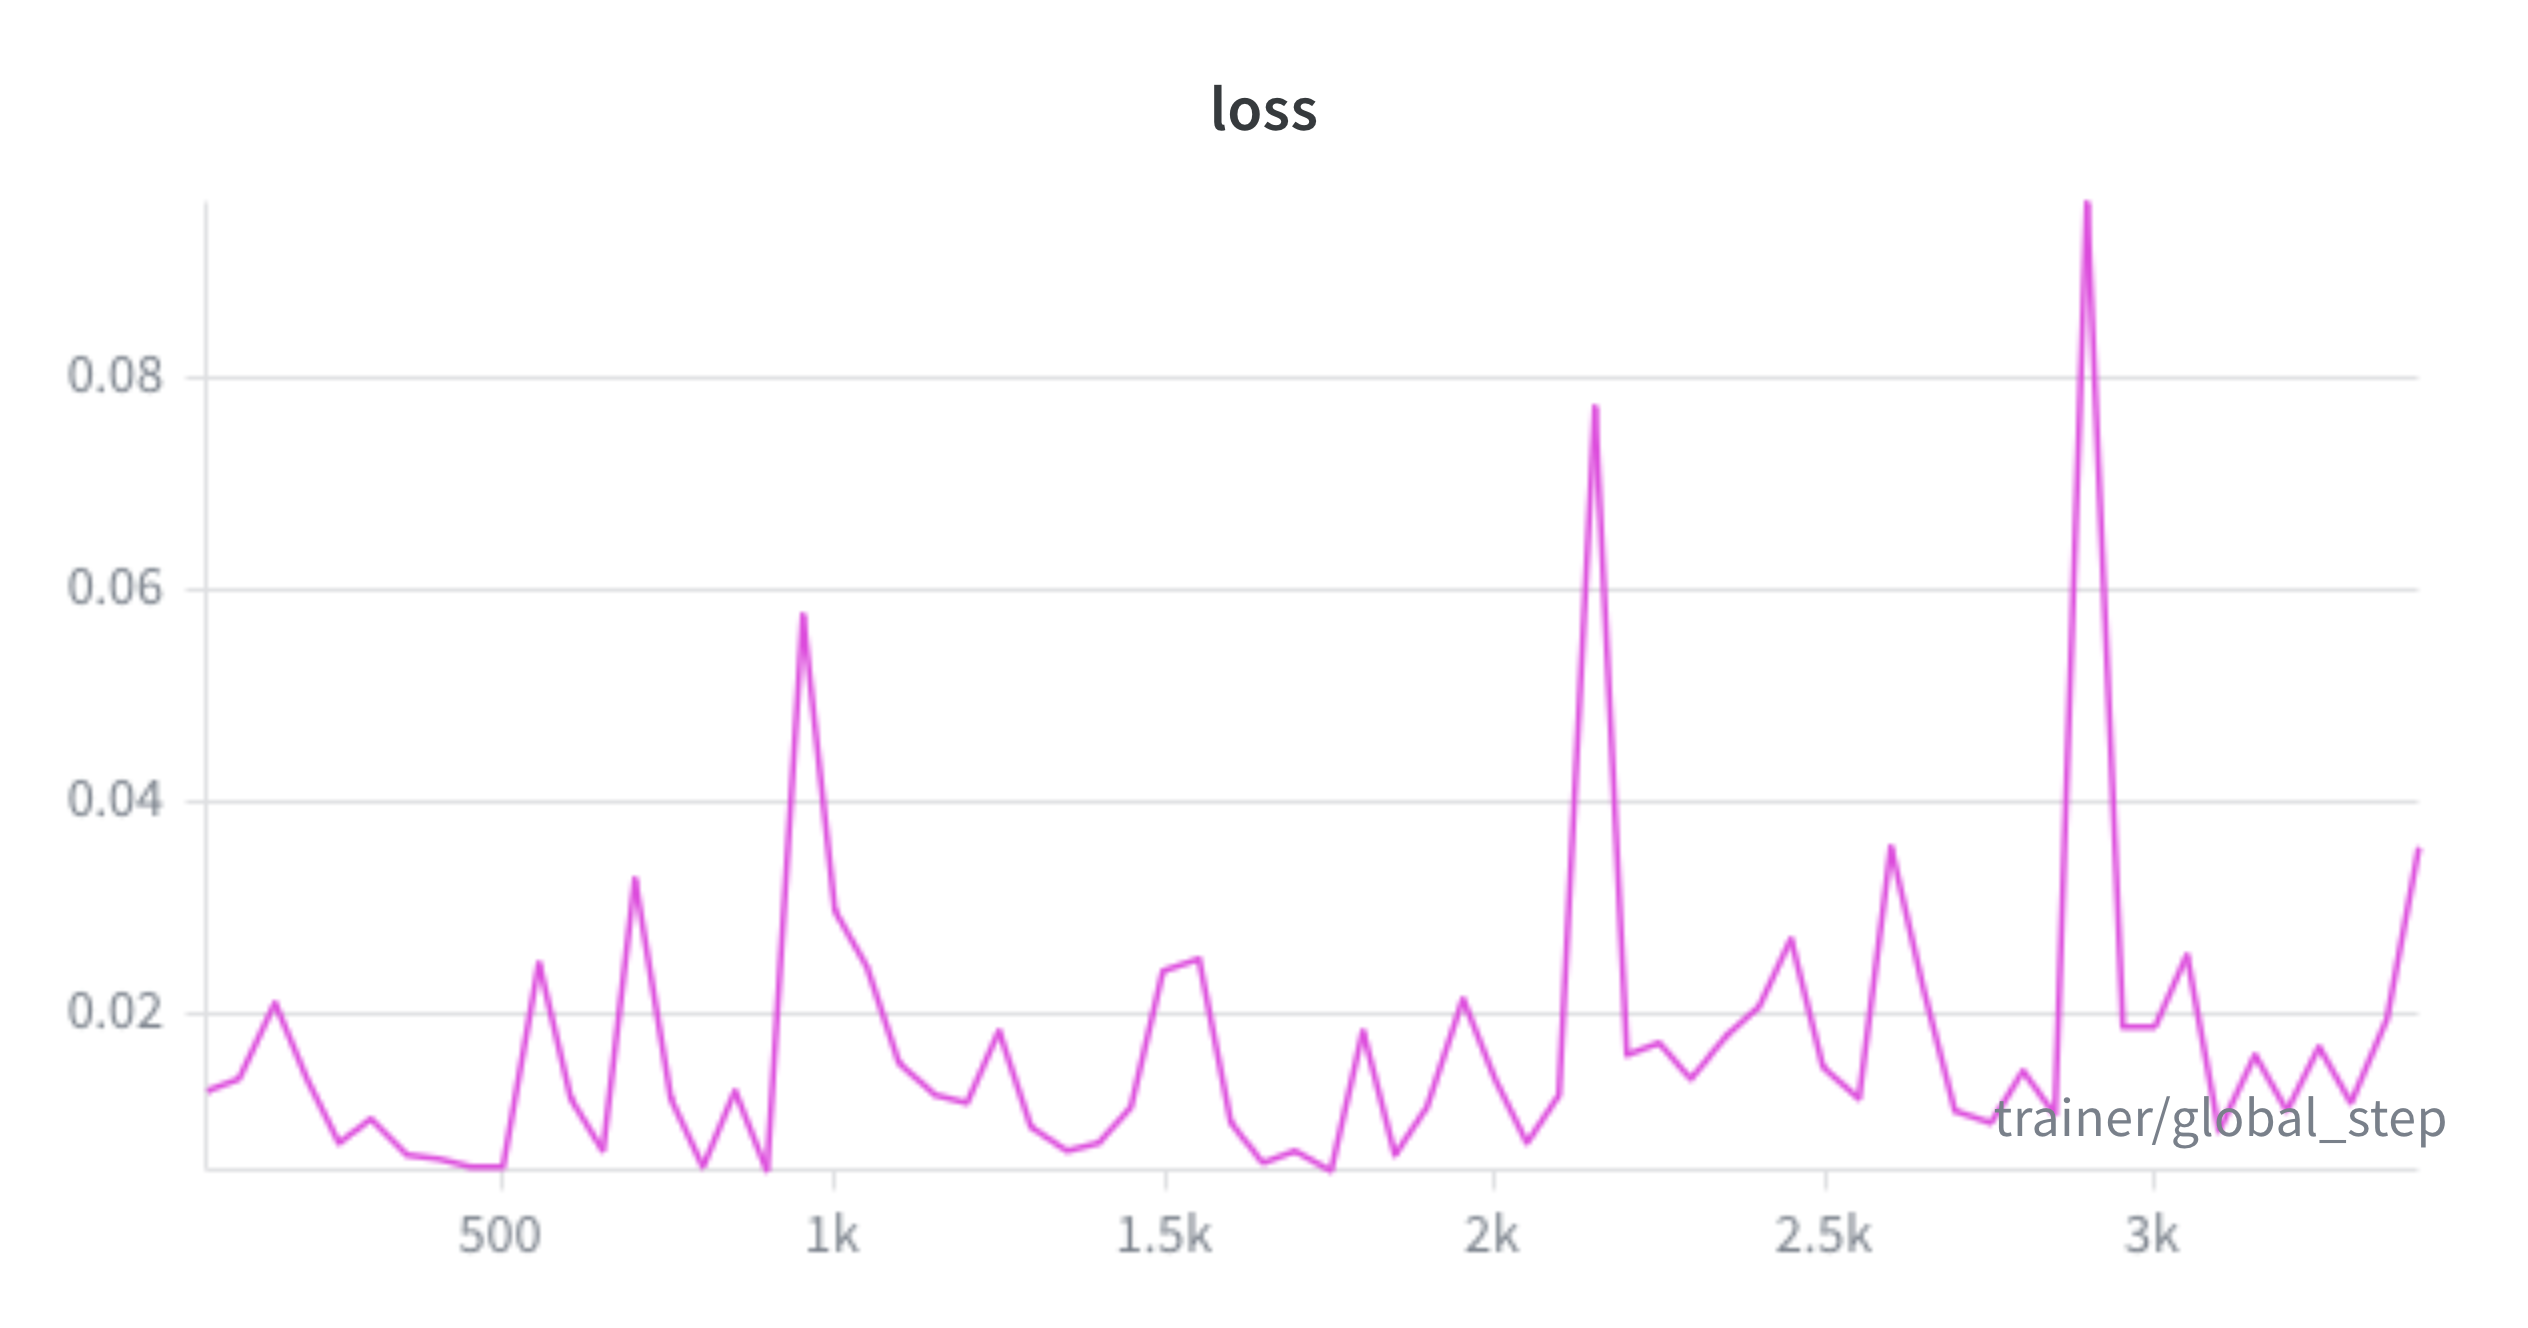
\includegraphics[width=5cm, height=4cm]{images/5-Experiments_and_results/Loss.png}
  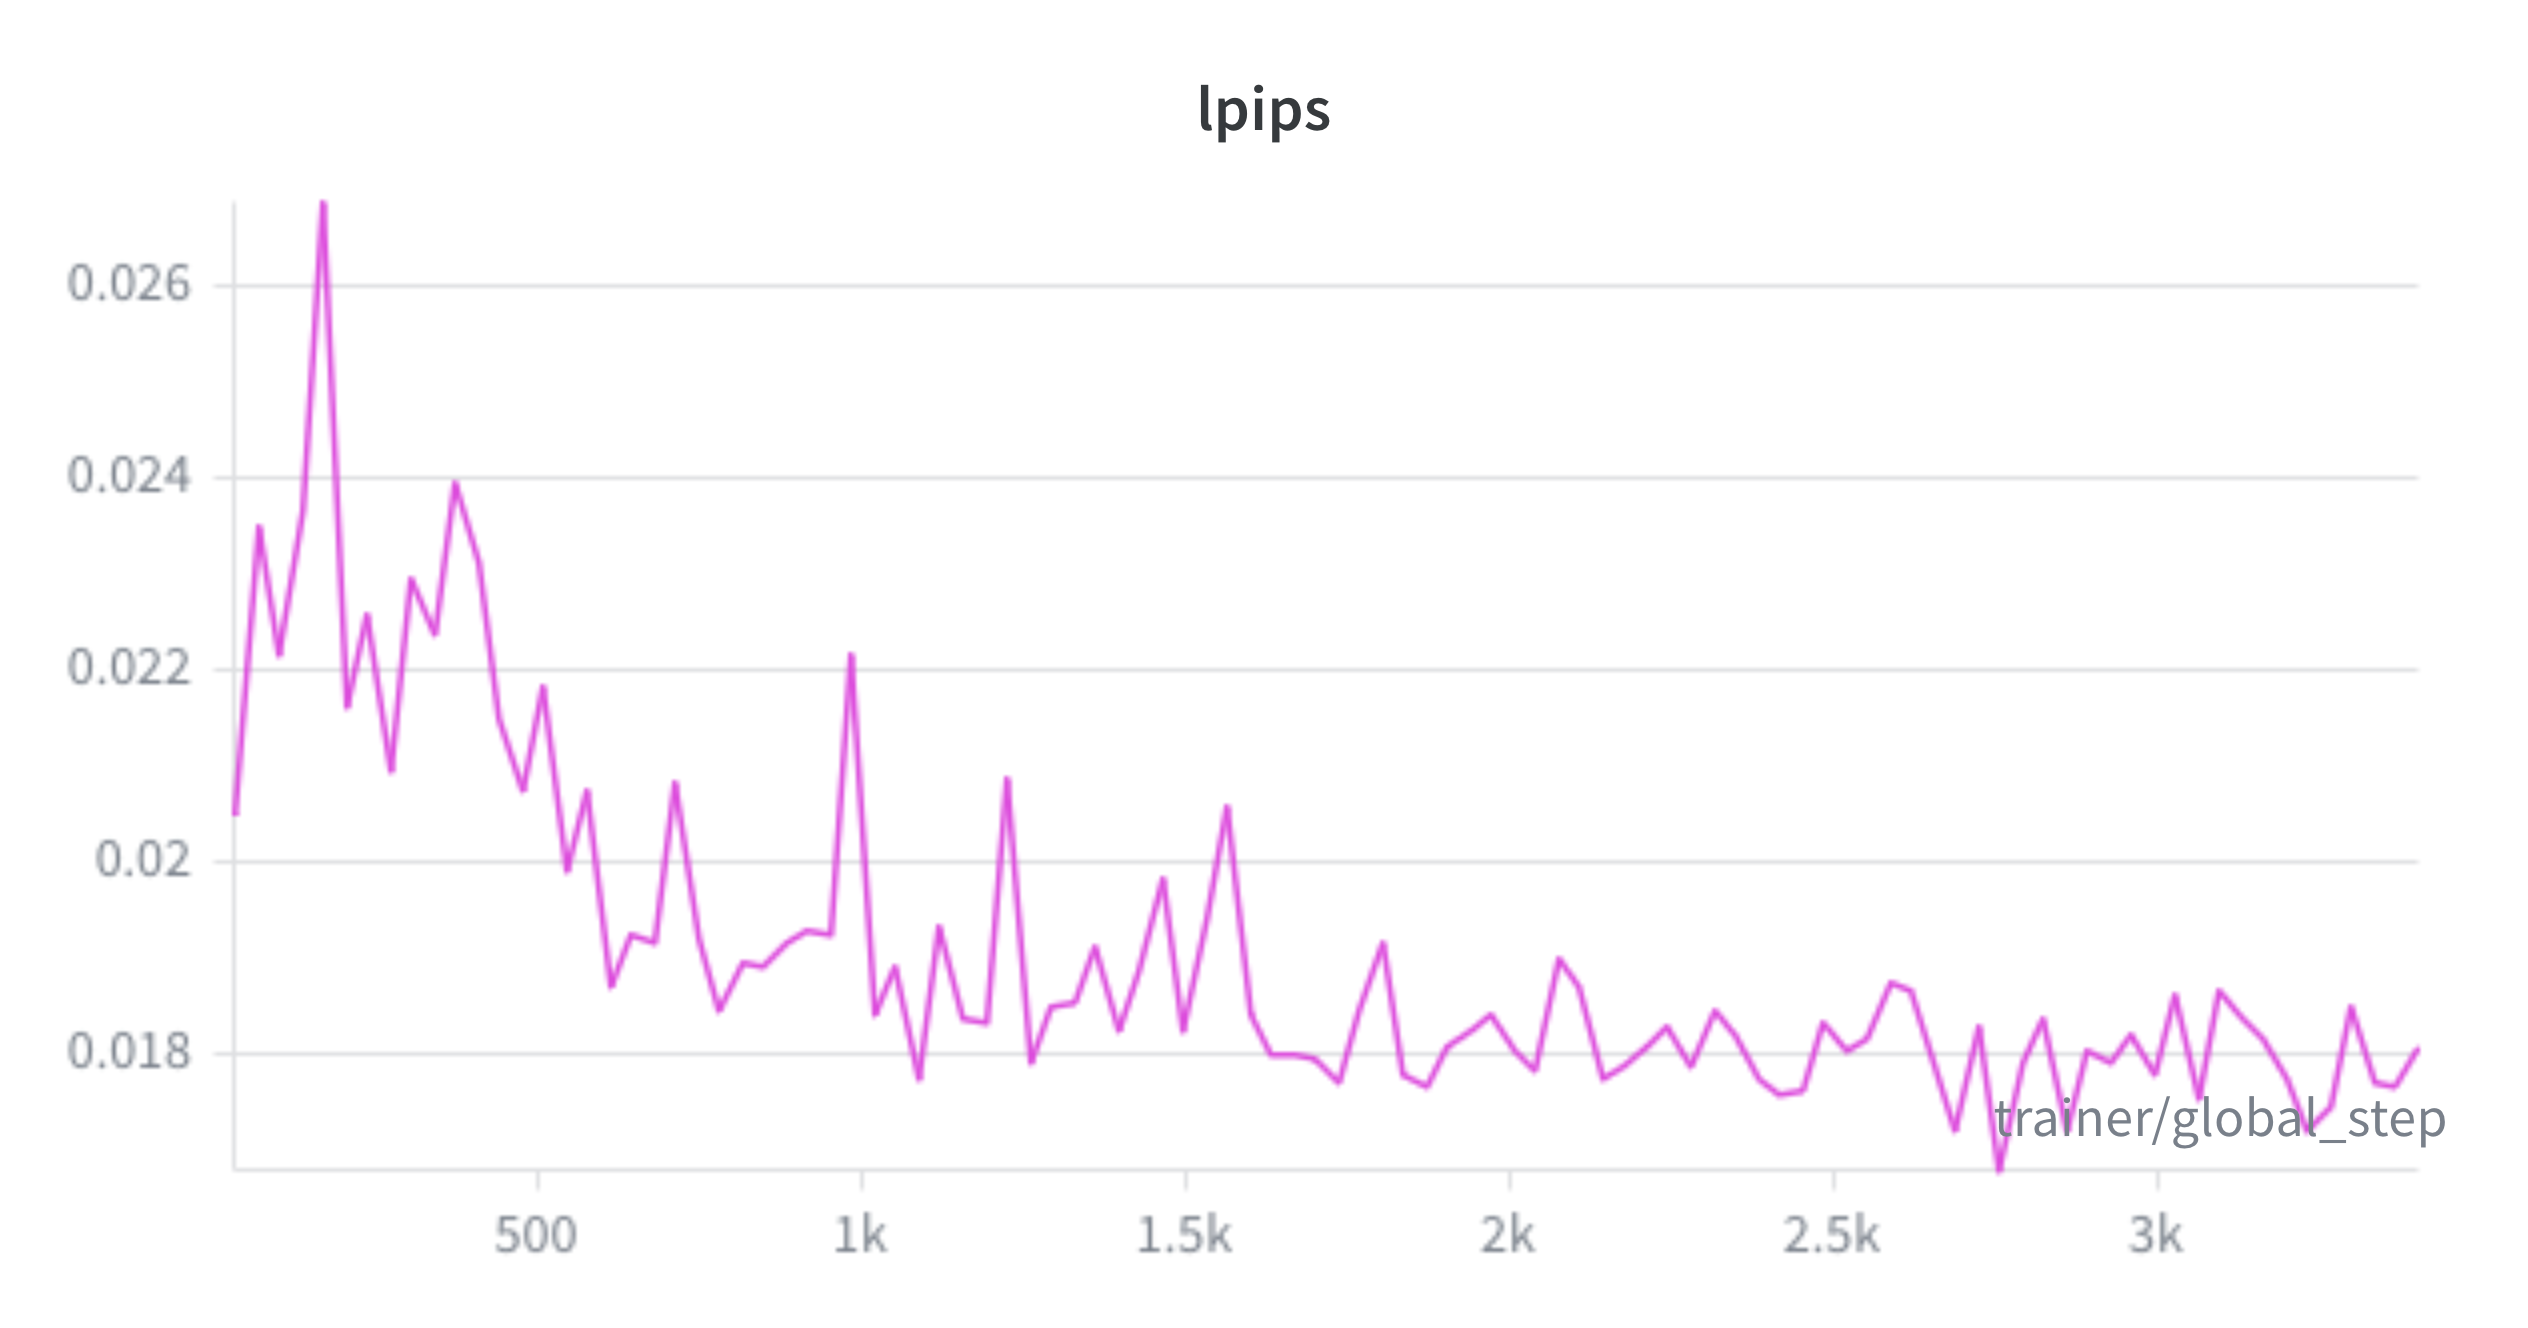
\includegraphics[width=5cm, height=4cm]{images/5-Experiments_and_results/LPIPS.png}
  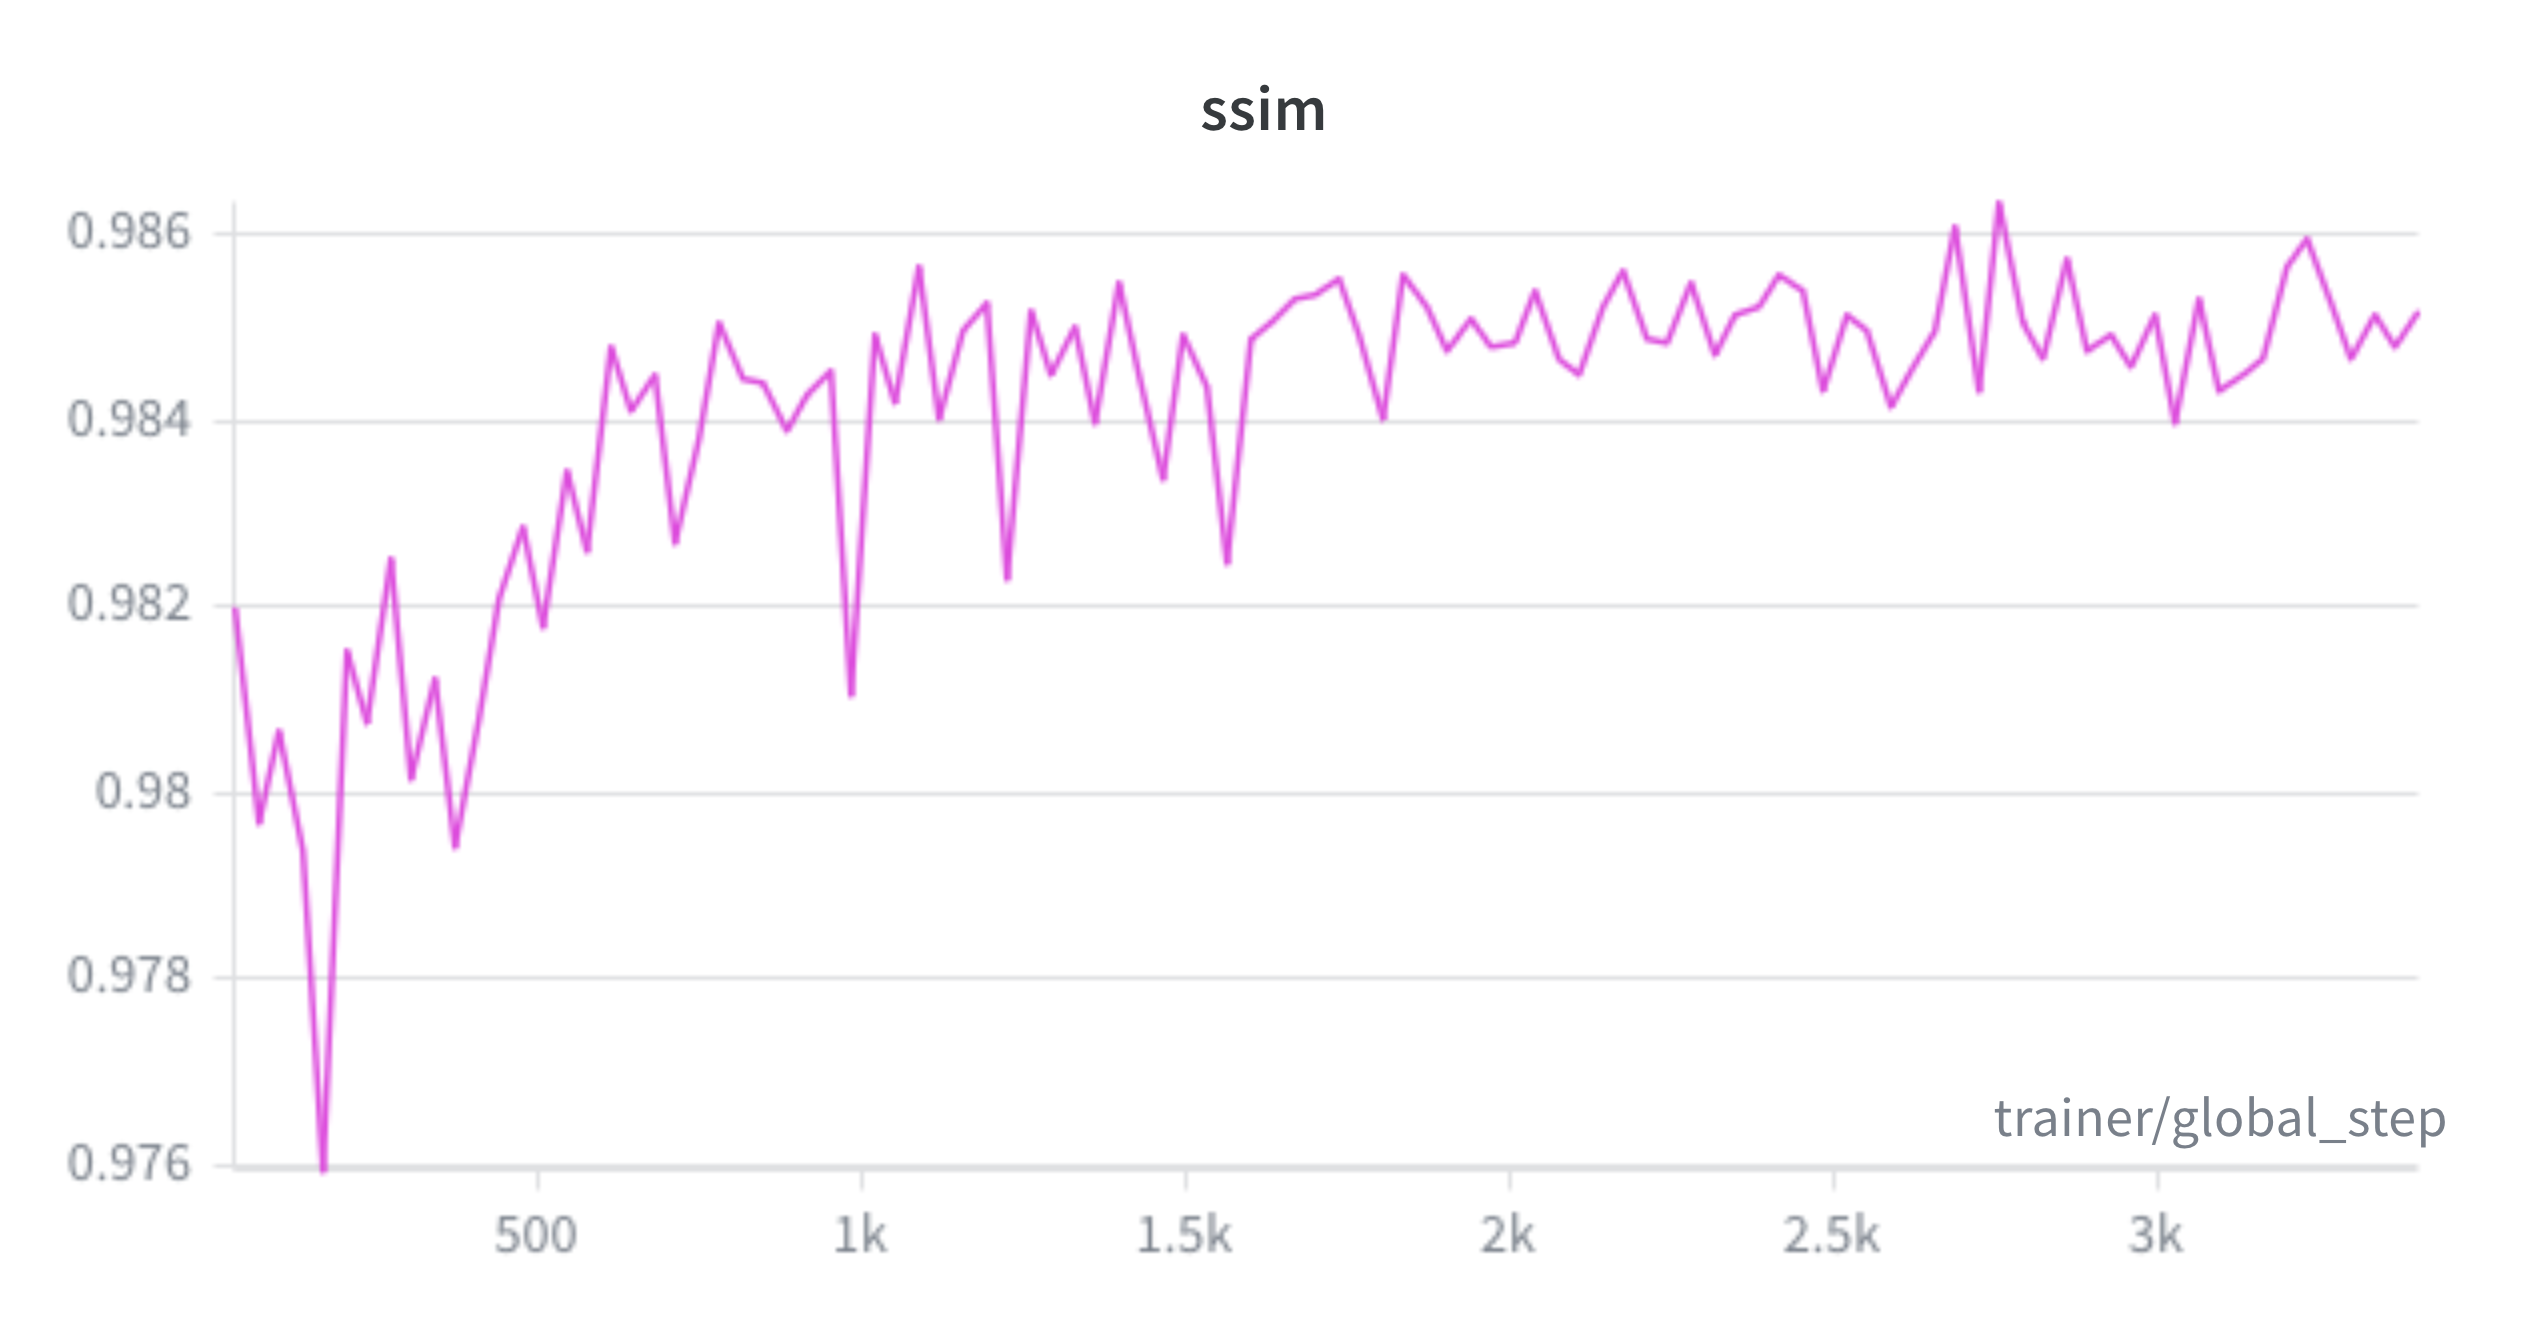
\includegraphics[width=5cm, height=4cm]{images/5-Experiments_and_results/SSIM.png}
  \caption{Courbe de la fonction de perte, de LPIPS et de SSIM de validation}
  \label{fig:courbe-loss-lpips-ssim}
\end{figure}


\section{Résultats par mouvement}

\subsection{Squat} \label{sec:resultats-squat}

Le squat constitue le mouvement le plus contraint visuellement, la barre chargée est portée sur le haut du dos, et les disques masquent en permanence une portion significative du torse, des épaules et parfois de la tête du sujet. Les montants du rack peuvent également apparaître en avant-plan dans la phase initiale du mouvement.

Le fine-tuning LoRA apporte une amélioration notable sur le squat (tableau~\ref{tab:resultats-squat}), avec une réduction de 24,5\,\% du LPIPS (0,0453 $\rightarrow$ 0,0342). Le gain en SSIM reste modéré (+0,43\,\%), ce qui est cohérent avec le comportement connu de cette métrique : le SSIM, fondé sur des statistiques locales de luminance et de contraste, est structurellement moins sensible aux différences de texture, de netteté des contours et de cohérence colorimétrique que LPIPS, dont les fonctionnalités profondes capturent davantage la plausibilité de la reconstruction.

\begin{table}[h]
  \centering
  \begin{tabular}{lccc}
    \hline
    \textbf{Modèle} & \textbf{SSIM} $\uparrow$ & \textbf{LPIPS} $\downarrow$ \\
    \hline
    TACO-baseline          & 0,977 & 0,0453 \\
    TACO-LoRA & \textbf{0,981} & \textbf{0,0342} \\
    \hline
  \end{tabular}
  \caption{Résultats quantitatifs sur la vidéo de \emph{squat}}
  \label{tab:resultats-squat}
\end{table}

\subsection{Développé couché} \label{sec:resultats-bench}

Le développé couché présente une géométrie d'occlusion particulière, la barre traverse horizontalement le champ de vision et masque le torse du sujet de façon quasi continue. La position allongée du sujet réduit également la surface visible exploitable comme indice de reconstruction.

Le développé couché présente l'amélioration la plus marquée de l'ensemble du jeu de données de test (tableau~\ref{tab:resultats-bench}), avec une réduction de 50,1\,\% du LPIPS (0,0792 $\rightarrow$ 0,0397) et un gain SSIM de 1,04\,\%. Ce résultat confirme l'hypothèse formulée au chapitre~\ref{ch_four} : l'occlusion quasi continue du torse constitue précisément le type de configuration pour lequel le fine-tuning spécialisé apporte le bénéfice le plus important. Le LPIPS baseline plus élevé (0,0792 contre 0,0453 au squat) reflète la difficulté intrinsèque de ce mouvement pour un modèle généraliste.

\begin{table}[h]
  \centering
  \begin{tabular}{lccc}
    \hline
    \textbf{Modèle} & \textbf{SSIM} $\uparrow$ & \textbf{LPIPS} $\downarrow$ \\
    \hline
    TACO-baseline          & 0,974 & 0,0792 \\
    TACO-LoRA & \textbf{0,984} & \textbf{0,0397} \\
    \hline
  \end{tabular}
  \caption{Résultats quantitatifs sur la vidéo de \emph{développé couché}}
  \label{tab:resultats-bench}
\end{table}

\subsection{Soulevé de terre} \label{sec:resultats-deadlift}

Le soulevé de terre offre une configuration intermédiaire, les disques sont visibles latéralement et masquent les jambes du sujet, mais le torse et la tête restent dégagés. La trajectoire verticale de la barre et la durée relativement courte des phases concentriques limitent la durée des occlusions.

Le soulevé de terre constitue le cas le moins favorable au fine-tuning (tableau~\ref{tab:resultats-deadlift}) : le LPIPS reste quasi identique entre le modèle baseline (0,0487) et le modèle fine-tuné (0,0489), soit une différence de 0,0002. Le gain SSIM est également très faible (+0,22\,\%). Ce résultat est cohérent avec les occlusions de ce mouvement : les disques masquent principalement les membres inférieurs latéralement, laissant le torse et la tête dégagés, ce qui limite l'apport du fine-tuning spécialisé.

\begin{table}[h]
  \centering
  \begin{tabular}{lccc}
    \hline
    \textbf{Modèle} & \textbf{SSIM} $\uparrow$ & \textbf{LPIPS} $\downarrow$ \\
    \hline
    TACO-baseline          & 0,959 & \textbf{0,0487} \\
    TACO-LoRA & \textbf{0,961} & 0,0489 \\
    \hline
  \end{tabular}
  \caption{Résultats quantitatifs sur la vidéo du \emph{soulevé de terre}}
  \label{tab:resultats-deadlift}
\end{table}

\section{Comparaison avant / après fine-tuning}

\subsection{Synthèse quantitative globale}

Le tableau~\ref{tab:resultats-globaux} agrège les résultats des trois mouvements et présente la performance moyenne sur l'ensemble du jeu de données de test.

\begin{table}[h]
  \centering
  \begin{tabular}{lccc}
    \hline
    \textbf{Modèle} & \textbf{SSIM} $\uparrow$ & \textbf{LPIPS} $\downarrow$ \\
    \hline
    TACO-baseline          & 0,970 & 0,0577 \\
    TACO-LoRA & 0,975 & 0,0375 \\
    \hline
    \textbf{Gain absolu}   & +0,005 & $-$0,020 \\
    \textbf{Gain relatif}  & +0,52\,\% & $-$35,0\,\% \\
    \hline
  \end{tabular}
  \caption{Résultats globaux sur l'ensemble du jeu de données de test (3 clips)}
  \label{tab:resultats-globaux}
\end{table}

Sur l'ensemble du jeu de données de test (1\,199 trames issues de 3 vidéos couvrant les trois mouvements de référence), le fine-tuning LoRA améliore le LPIPS de 35,0\,\% en moyenne. Le gain en SSIM est plus modeste (+0,52\,\%), ce qui est attendu, LPIPS est davantage aligné avec la perception humaine de la qualité de reconstruction que le SSIM, qui opère sur des statistiques locales de luminance et de contraste.

\subsection{Significativité statistique}

Pour vérifier que les écarts observés entre le modèle baseline et le modèle fine-tuné ne sont pas attribuables au hasard, un test de Wilcoxon apparié~\cite{Wilcoxon-1945} est conduit trame par trame sur les 1\,199 trames du jeux de données de test. Les valeurs $p$ obtenues sont les suivantes :

\begin{itemize}
  \item SSIM  : $p = 1{,}45 \times 10^{-96}$
  \item LPIPS : $p = 3{,}28 \times 10^{-5}$
\end{itemize}

Les deux tests rejettent l'hypothèse nulle avec $\alpha = 0{,}05$. Ces résultats doivent néanmoins être interprétés avec précaution : les 1\,199 trames provenant de seulement 3 vidéos d'un unique sujet, les observations ne sont pas strictement indépendantes (corrélation temporelle intra-vidéo), ce qui tend à gonfler artificiellement la significativité statistique. Ces résultats sont donc indicatifs plutôt que conclusifs, et devront être confirmés sur un jeu de données de test plus large et plus diversifié.

\subsection{Analyse qualitative comparative}

Les figures~\ref{fig:qual-squat}, \ref{fig:qual-bench} et \ref{fig:qual-deadlift} présentent, pour chacun des trois mouvements, une trame représentative sous quatre conditions : référence non-occluse (A), entrée occluse (B), reconstruction TACO-baseline (C), reconstruction TACO-LoRA (D).

Au squat (figure~\ref{fig:qual-squat}), l'occlusion porte principalement sur l'épaule droite et la partie supérieure du torse, masquées par le disque. TACO-baseline produit une reconstruction de l'épaule et du torse floue avec une colorimétrie dégradée du \textit{singlet}. TACO-LoRA restitue une silhouette plus nette et une continuité du tissu cohérente avec les trames adjacentes.

\begin{figure}[htp]
  \centering
  
\includegraphics[width=3cm, height=5cm]{images/5-Experiments_and_results/Squat.png}
  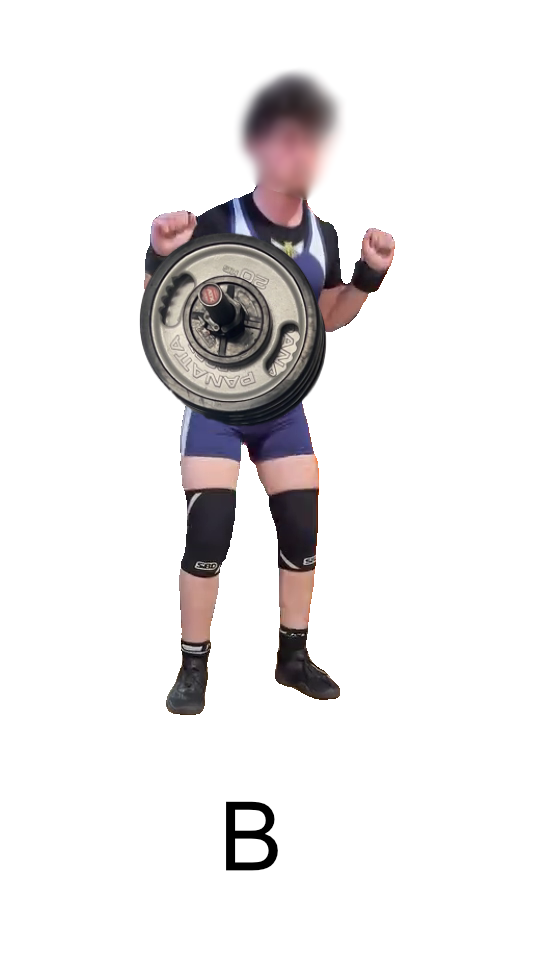
\includegraphics[width=3cm, height=5cm]{images/5-Experiments_and_results/Squat-occlusion.png}
  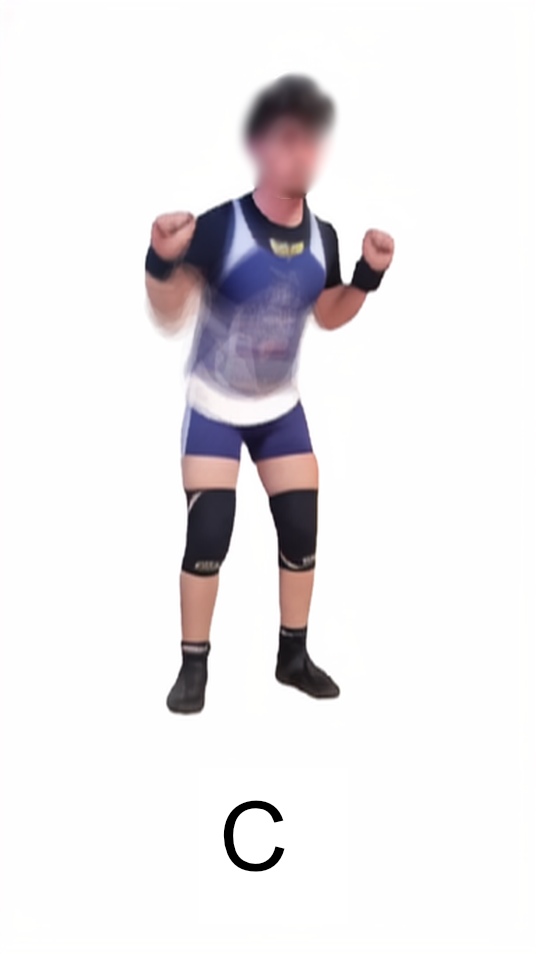
\includegraphics[width=3cm, height=5cm]{images/5-Experiments_and_results/Squat-baseline.png}
  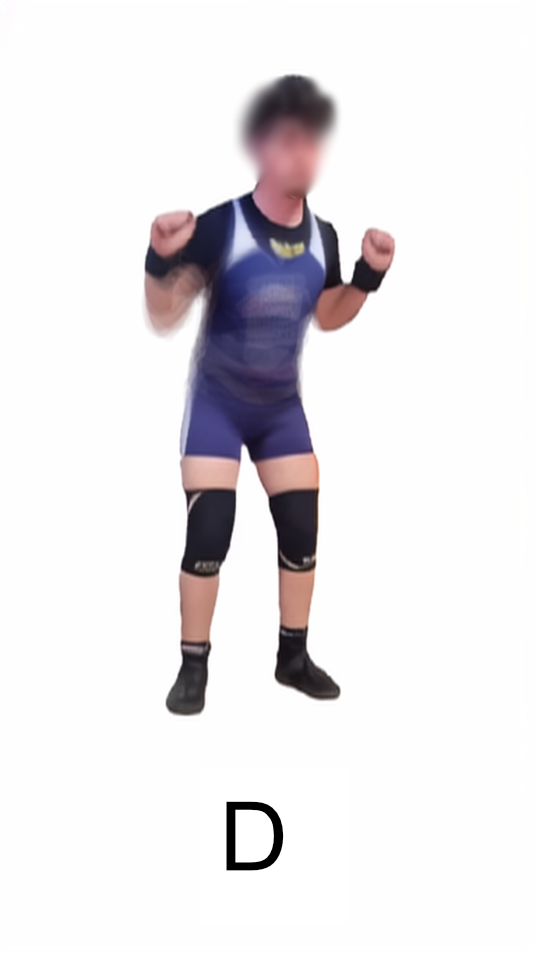
\includegraphics[width=3cm, height=5cm]{images/5-Experiments_and_results/Squat-lora.png}
  \caption{Comparaisons visuelles au squat}
  \label{fig:qual-squat}
\end{figure}

Au développé couché (figure~\ref{fig:qual-bench}), la sécurité masque quasi intégralement le torse sur toute la durée du mouvement. TACO-baseline laisse subsister une zone grisée incohérente au centre de la reconstruction, révélant une incertitude élevée du modèle généraliste face à cette situation. TACO-LoRA produit un torse reconstruit plus plausible, avec une continuité de l'habillement préservée entre les trames consécutives. Ce contraste est cohérent avec la réduction de 50,1\,\% du LPIPS observée sur ce mouvement.

\begin{figure}[htp]
  \centering
  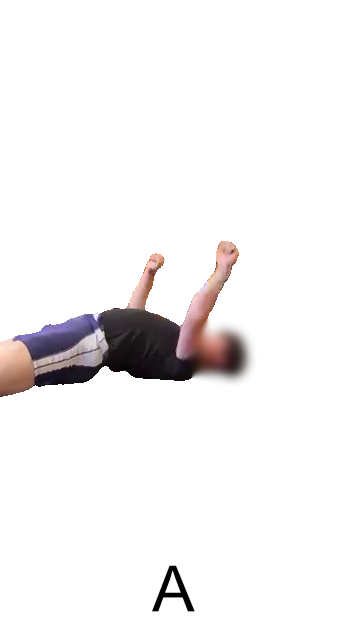
\includegraphics[width=3cm, height=5cm]{images/5-Experiments_and_results/Bench.png}
  
\includegraphics[width=3cm, height=5cm]{images/5-Experiments_and_results/Bench-occlusion.png}
  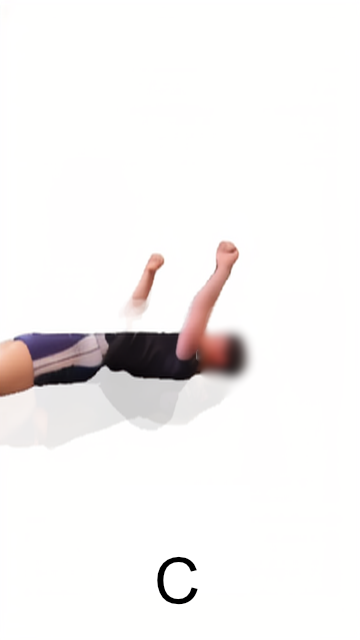
\includegraphics[width=3cm, height=5cm]{images/5-Experiments_and_results/Bench-baseline.png}
  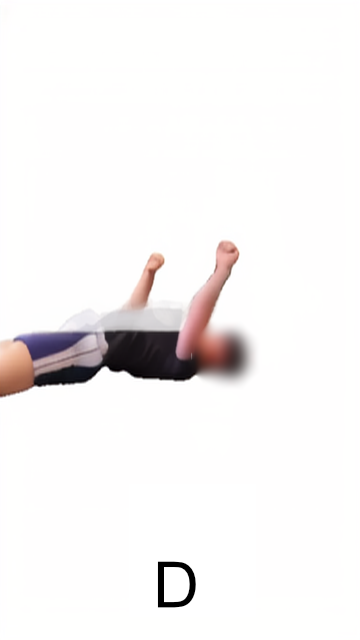
\includegraphics[width=3cm, height=5cm]{images/5-Experiments_and_results/Bench-lora.png}
  \caption{Comparaisons visuelles au développé couché}
  \label{fig:qual-bench}
\end{figure}

Au soulevé de terre (figure~\ref{fig:qual-deadlift}), le disque masque la région pelvienne et le haut des cuisses. Les reconstructions TACO-baseline et TACO-LoRA sont visuellement proches, ce qui est cohérent avec l'absence d'amélioration métrique significative sur ce mouvement ($\Delta$LPIPS = +0,0002).

\begin{figure}[htp]
  \centering
  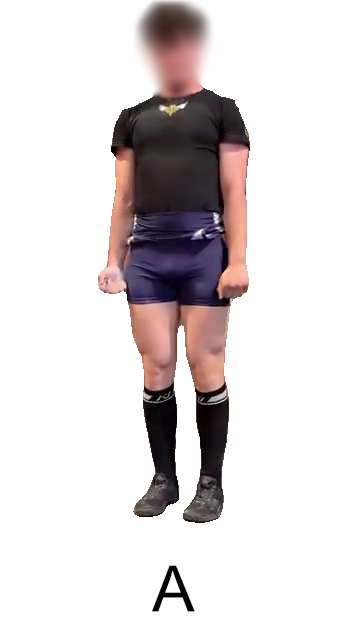
\includegraphics[width=3cm, height=5cm]{images/5-Experiments_and_results/Deadlift.png}
  
\includegraphics[width=3cm, height=5cm]{images/5-Experiments_and_results/Deadlift-occlusion.png}
  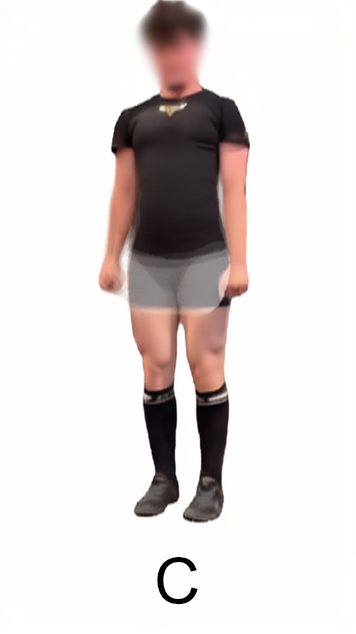
\includegraphics[width=3cm, height=5cm]{images/5-Experiments_and_results/Deadlift-baseline.png}
  
\includegraphics[width=3cm, height=5cm]{images/5-Experiments_and_results/Deadlift-lora.png}
  \caption{Comparaisons visuelles au soulevé de terre}
  \label{fig:qual-deadlift}
\end{figure}

\section{Analyse du cas limite}

\subsection{Occlusions massives et prolongées}

Lorsque la part occluse dépasse approximativement 60\,\% du sujet (figure~\ref{fig:big-occlusion-limitation}) sur une fenêtre temporelle longue (au-delà de la fenêtre d'inférence native de 14 trames de TACO, le modèle perd les indices visuels nécessaires à une reconstruction fidèle et tend à produire des solutions "hallucinées" plausibles mais infidèles~\cite{TACO-2025}). Le cas typique est celui d'un développé couché vu de côté où les disques cachent intégralement les bras du sujet sur l'ensemble du mouvement concentrique. Une stratégie d'atténuation envisagée est la propagation explicite d'informations depuis les trames pré- et post-occlusion via un mécanisme d'attention étendue, à l'image de l'approche proposée par ProPainter~\cite{ProPainter-2023}.

\begin{figure}[htp]
  \centering
  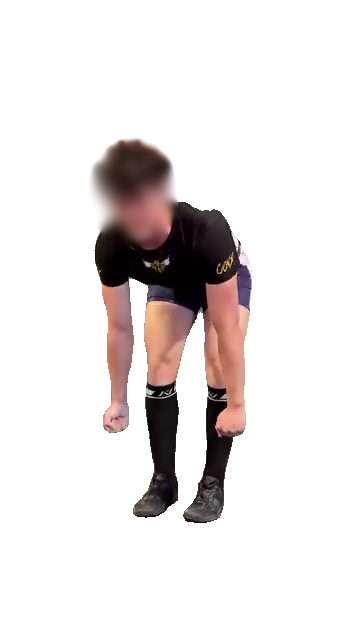
\includegraphics[width=3cm, height=5cm]{images/5-Experiments_and_results/Big-occlusion-frame.png}
  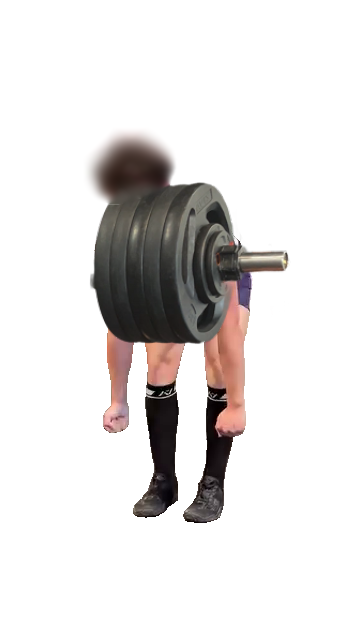
\includegraphics[width=3cm, height=5cm]{images/5-Experiments_and_results/Big-occlusion-frame-occluded.png}
  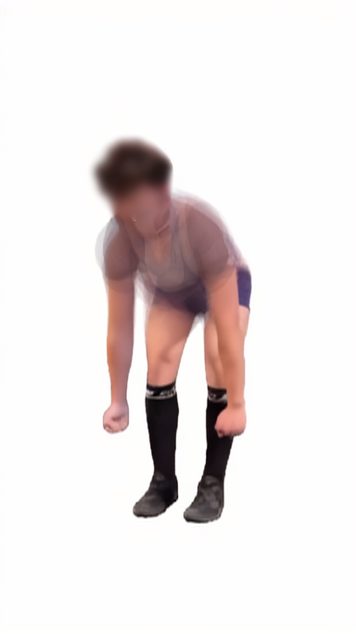
\includegraphics[width=3cm, height=5cm]{images/5-Experiments_and_results/Big-occlusion-frame-lora.png}
  \caption{Hallucination avec une occlusion massive et prolongée}
  \label{fig:big-occlusion-limitation}
\end{figure}

\section{Discussion et comparaison à l'état de l'art}

\subsection{Positionnement par rapport à TACO original}

Les auteurs de TACO rapportent, sur leur benchmark OvO-Hard, un LPIPS moyen de 0,142~\cite{TACO-2025} sur des séquences d'objets génériques. Sur le benchmark powerlifting, le modèle baseline atteint 0,058 en LPIPS moyen, une valeur nettement inférieure qui s'explique par la nature du domaine : les séquences de force athlétique du dataset présentent un sujet isolé sur fond blanc, une géométrie d'occlusion répétitive et des textures vestimentaires relativement homogènes, ces conditions sont plus favorables que les objets génériques du dataset OvO.

Après fine-tuning LoRA, notre modèle atteint 0,038 en LPIPS, soit une amélioration de 35,0\,\% sur le domaine ciblé. C'est cohérent avec ce que la littérature rapporte pour des fine-tunings LoRA spécialisés sur des modèles de diffusion vidéo~\cite{LoRA-2021} : on rapporte des gains de l'ordre de 20 à 40\,\% sur des tâches de génération spécialisées avec des rangs comparables ($r = 16$), et des travaux appliquant LoRA à Stable Diffusion pour des domaines visuels restreints confirment qu'un dataset de quelques dizaines de séquences suffit à produire une adaptation significative lorsque le modèle de base est déjà bien initialisé~\cite{DreamBooth-2023}.

\subsection{Comparaison avec les alternatives discutées}

Une comparaison formelle avec pix2gestalt et ProPainter n'a pas été conduite dans ce travail. Les arguments avancés au chapitre~\ref{ch_three} restent donc indicatifs plutôt que quantitativement validés. Néanmoins, les résultats obtenus sur TACO permettent de formuler deux observations.

D'une part, la cohérence temporelle native de TACO constitue un avantage structurel difficile à quantifier sur une métrique trame-à-trame comme LPIPS, mais visible qualitativement dans la stabilité des reconstructions entre trames consécutives. D'autre part, ProPainter~\cite{ProPainter-2023} requiert les masques d'occlusion en entrée, ce qui suppose de savoir a priori quelles régions du sujet sont masquées, un problème que TACO résout précisément via la complétion amodale. Une comparaison directe entre les deux méthodes constitue une perspective pour les travaux futurs.

\section{Résultats et Discussion} \label{sec:implications-pipeline}

Le tableau~\ref{tab:mpjpe} présente le MPJPE (\textit{Mean Per-Joint Position Error}) calculé entre la reconstruction 3D produite par SAM 3D Body sur les images de référence avant l'occlusion (\textit{ground truth}), les images occluses brutes, les sorties TACO-baseline, et les sorties TACO-LoRA.

\begin{table}[h]
  \centering
  \begin{tabular}{lccc}
    \hline
    \textbf{Mouvement} & \textbf{Occlus} & \textbf{TACO-baseline} & \textbf{TACO-LoRA} \\
                       & MPJPE (mm)      & MPJPE (mm)             & MPJPE (mm) \\
    \hline
    Squat              & $\mathbf{43{,}7 \pm 26{,}5}$ & $48{,}0 \pm 21{,}1$ & $47{,}3 \pm 21{,}5$ \\
    Développé couché   & $38{,}0 \pm 24{,}1$ & $43{,}4 \pm 21{,}1$ & $\mathbf{37{,}2 \pm 17{,}6}$ \\
    Soulevé de terre   & $\mathbf{94{,}3 \pm 40{,}1}$ & $181{,}8 \pm 143{,}1$ & $108{,}0 \pm 54{,}2$ \\
    \hline
  \end{tabular}
  \caption{MPJPE (mm) entre la reconstruction 3D et le ground truth, pour les trois conditions d'entrée de SAM 3D Body. Les valeurs indiquent la moyenne ainsi que l'écart-type ($\pm$) sur l'ensemble des trames de chaque mouvement.}
  \label{tab:mpjpe}
\end{table}

La figure~\ref{fig:mpjpe-boxplot} présente la distribution du MPJPE sous forme de boîtes à moustaches, révélant non seulement les tendances centrales mais également la dispersion et la présence de valeurs extrèmes pour chaque condition.

\begin{figure}[htp]
  \centering
  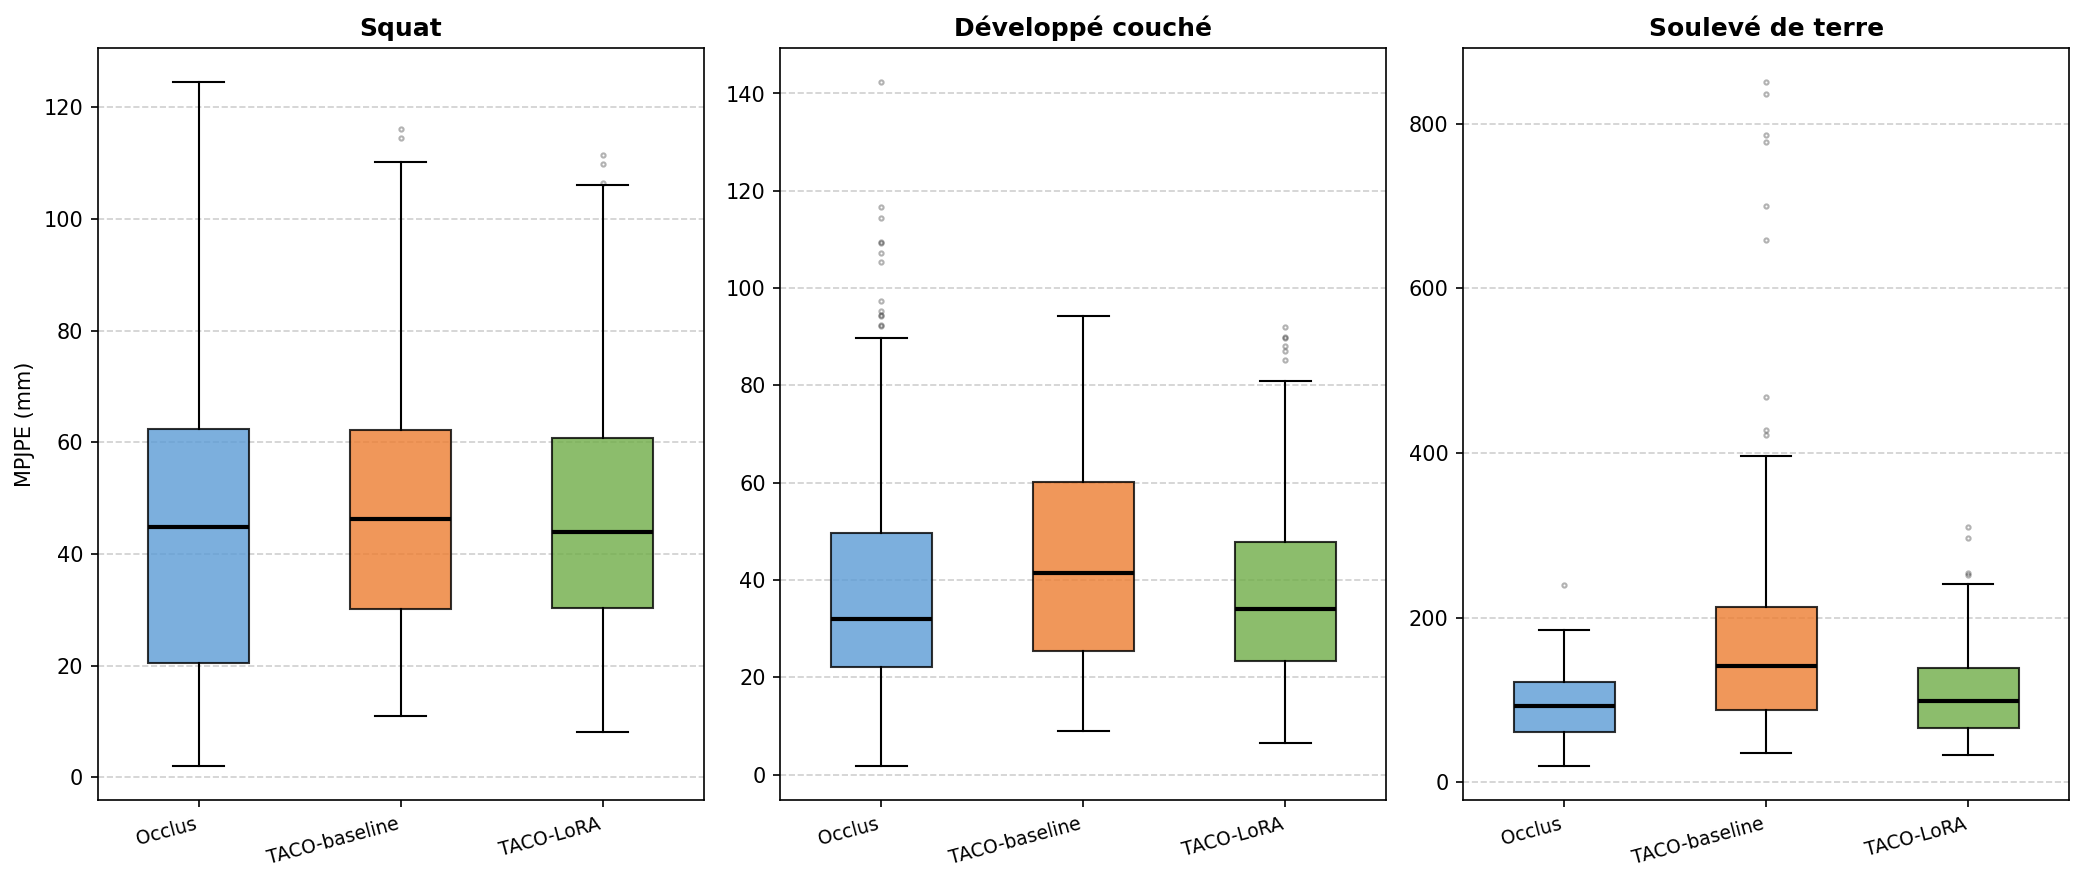
\includegraphics[width=14cm, height=6.5cm]{images/5-Experiments_and_results/mpjpe-boxplot.png}
  \caption{Distribution du MPJPE pour les trois conditions d'entrée de SAM 3D Body}
  \label{fig:mpjpe-boxplot}
\end{figure}

Trois observations se dégagent. Premièrement, au développé couché, TACO-LoRA atteint un MPJPE de 37,2~mm, légèrement inférieur à celui obtenu sur l'image occluse brute (38,0~mm), confirmant que la complétion amodale améliore effectivement la reconstruction 3D sur ce mouvement. Deuxièmement, au soulevé de terre, TACO-baseline produit une erreur particulièrement élevée (181,8~mm, avec un écart-type de 143~mm révélateur d'une forte instabilité), tandis que TACO-LoRA ramène cette erreur à 108,0~mm, soit une réduction de 40,6\,\% par rapport au baseline. Ce résultat suggère que le fine-tuning spécialisé stabilise les reconstructions dans les configurations d'occlusion les plus difficiles pour le modèle généraliste. Troisièmement, au squat, l'amélioration apportée par TACO-LoRA reste marginale ($-$0,7~mm par rapport au baseline), cohérente avec les résultats 2D de la section~\ref{sec:resultats-squat}.

Il convient de noter que, pour les trois mouvements, TACO-LoRA n'améliore pas systématiquement le MPJPE par rapport à l'image occluse brute (+3,6~mm au squat, +13,7~mm au soulevé de terre). Ce résultat indique que la complétion amodale, même améliorée par le fine-tuning, peut introduire des artefacts visuels suffisamment importants pour perturber SAM 3D Body davantage que l'occlusion originale. Cette limite est discutée dans la section~\ref{sec:limites}.

\medskip
Le chapitre suivant tire les conclusions générales de ce travail et identifie les pistes d'amélioration et d'extension les plus prometteuses pour la suite du développement de ce pipeline.